\documentclass[11pt,a4paper]{article}
\usepackage[utf8]{inputenc}
\usepackage[margin=0.75in]{geometry}
\setlength{\headheight}{14pt}
\usepackage{graphicx}
\usepackage{amsmath,amssymb}
\usepackage{booktabs}
\usepackage{longtable}
\usepackage{array}
\usepackage{hyperref}
\usepackage{float}
\usepackage{caption}
\usepackage{subcaption}
\usepackage{fancyhdr}
\usepackage{titlesec}
\usepackage{xcolor}

% Custom Colors matching previous reports
\definecolor{primary}{RGB}{0, 51, 102}
\definecolor{secondary}{RGB}{70, 130, 180}

\hypersetup{
    colorlinks=true,
    linkcolor=primary,
    citecolor=primary,
    urlcolor=secondary
}

% Header and Footer setup
\pagestyle{fancy}
\fancyhf{}
\rhead{\textcolor{primary}{\textbf{EDC Laboratory --- Experiment 7}}}
\lhead{\textcolor{primary}{\textbf{EE25BTECH11056 \& EE25BTECH11049}}}
\rfoot{Page \thepage}

\titleformat{\section}{\large\bfseries\color{primary}}{\thesection.}{0.5em}{}
\titleformat{\subsection}{\normalfont\bfseries\color{secondary}}{\thesubsection}{0.5em}{}
\titleformat{\subsubsection}{\normalfont\bfseries}{\thesubsubsection}{0.5em}{}

\begin{document}

% Title Page / Header Block
\begin{center}
    {\LARGE \textbf{\color{primary} DEPARTMENT OF ELECTRICAL ENGINEERING}}\\[0.2cm]
    {\large \textbf{Electronic Devices \& Circuits Laboratory (EDC LAB)}}\\[0.4cm]
    \rule{\linewidth}{1pt}\\[0.3cm]
    {\Large \textbf{EXPERIMENT 7: NMOS Source Follower with Current-Mirror Load}}\\[0.3cm]
    \rule{\linewidth}{1pt}\\[0.4cm]
    
    \begin{tabular}{ll}
        \textbf{Prepared By:} & \textbf{Suraj.N (EE25BTECH11056)} \\
                              & \textbf{Sai Krishna Bakki (EE25BTECH11049)} \\
        \textbf{Course:}      & Electronic Devices \& Circuits Lab \\
        \textbf{Date:}        & \today
    \end{tabular}
\end{center}

\vspace{0.2cm}

\section{Aim and Objectives}
\begin{enumerate}
    \item To assemble a simple NMOS source follower (common-drain amplifier) biased by an active current-source load built from a current mirror.
    \item To characterize its DC transfer function, small-signal voltage gain, and output resistance.
    \item To verify that a current-source-loaded follower provides near-unity gain, wide linear swing, and very low output resistance even at moderate bias currents.
\end{enumerate}

\section{Apparatus and Circuit Specifications}
\begin{table}[H]
\centering
\caption{Equipment and Components Used in Experiment}
\begin{tabular}{@{}cllp{6.5cm}@{}}
\toprule
\textbf{S.No.} & \textbf{Component / Equipment} & \textbf{Value / Specification} & \textbf{Purpose / Operating Note} \\ \midrule
1 & Dual N-Channel MOSFET & SI9926BDY (SO-8 to DIP-8) & $M_{ref}, M_{cs}, M_{sf}$ channels used \\
2 & Reference Resistor $R_{ref}$ & $270\ \Omega$, $\pm 5\%$ & Sets reference current $I_{ref} \approx 40\text{ mA}$ \\
3 & Potentiometer & $10\text{ k}\Omega$ multi-turn & Input DC bias divider for $V_{in}$ \\
4 & DC Decoupling Resistor & $1\text{ M}\Omega$ & Isolates AC signal path from bias potentiometer \\
5 & Coupling Capacitor $C_{in}$ & $1\ \mu\text{F}$ & AC-couples function generator onto DC-biased gate \\
6 & Load Resistors & $22\ \Omega, 47\ \Omega, 56\ \Omega, 82\ \Omega$ & Used for $R_{out}$ loading measurements \\
7 & DC Power Supply & $0-30\text{ V}$ regulated & Set to $V_{DD} = 12\text{ V}$, current-limited at $150\text{ mA}$ \\
8 & Function Generator & Sine output, $10\text{ Hz} - 100\text{ kHz}$ & Small amplitude AC source for frequency response \\
9 & Oscilloscope \& DMM & 2-channel, Precision 4.5 digit & To record $V_{in}, V_{out}$ amplitudes and DC voltages \\
\bottomrule
\end{tabular}
\end{table}

\subsection{Pin Configuration and Schematic Diagram}
The SI9926BDY dual TrenchFET resides in an SO-8 package mounted on a DIP-8 breakout board. 
$M_{ref}$ (diode-connected) and $R_{ref}$ set a reference current $I_{ref} \approx 40\text{ mA}$. $M_{ref}$'s gate drives $M_{cs}$, mirroring the current $1:1$ to form an active current-source load at the output node. $M_{sf}$, the source follower, has its drain tied to $V_{DD} = 12\text{ V}$ and its source tied to this active load.

\begin{figure}[H]
    \centering
    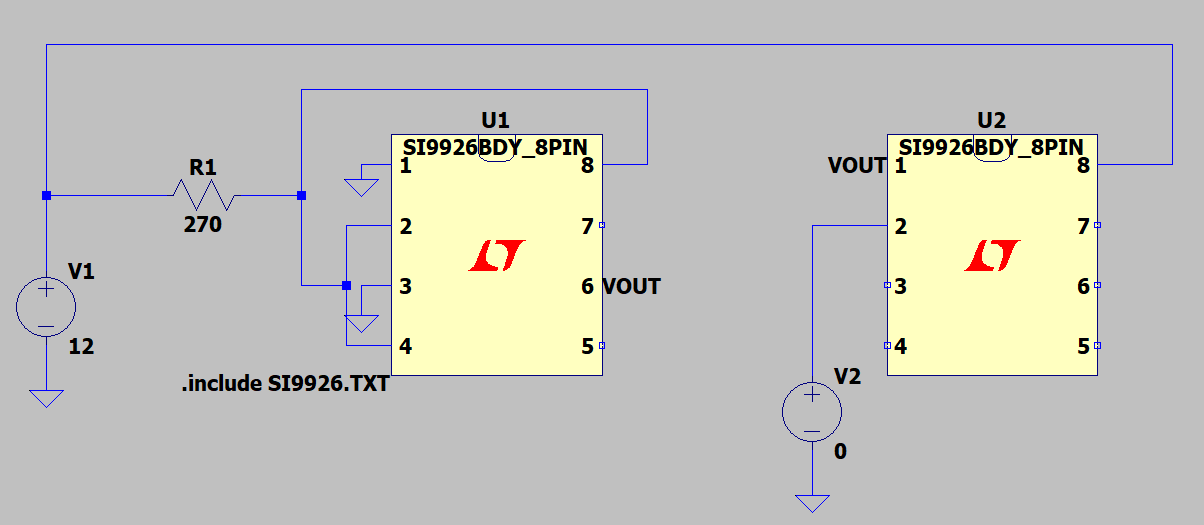
\includegraphics[width=0.75\textwidth]{Schematic.png}
    \caption{Circuit Schematic of the NMOS Source Follower with Current-Mirror Load.}
    \label{fig:schematic}
\end{figure}

\section{Theoretical Framework}
\subsection{DC Transfer Characteristic}
Because $M_{cs}$'s gate is fixed (tied to the mirror reference), the current it sinks is fixed at $I_{ref}$ regardless of $V_{in}$. Since $M_{sf}$ and $M_{cs}$ form the only two current paths into the output node, $M_{sf}$ must also carry exactly this same fixed current at all times. This forces $M_{sf}$'s $V_{GS}$ to a constant value, independent of $V_{in}$. The DC transfer characteristic is therefore simply:
\begin{equation}
    V_{out} = V_{in} - V_{GS}(M_{sf})
\end{equation}
with $V_{GS}(M_{sf})$ fixed by $I_{ref}$ --- an exact unity-slope, level-shifted line.

\subsection{Small-Signal Voltage Gain}
The small-signal voltage gain follows the same reasoning:
\begin{equation}
    A_v = \frac{dV_{out}}{dV_{in}} = \frac{g_m}{g_m + \frac{1}{r_{o,total}}} \approx 1
\end{equation}
for high transconductance $g_m$ and high incremental output resistance $r_{o,total} = r_{o,sf} \parallel r_{o,cs}$ of the active current-source load.

\subsection{Output Resistance}
The output resistance looking back into $V_{out}$ is approximately:
\begin{equation}
    R_{out} \approx \frac{1}{g_m}
\end{equation}
Because the device operates in the weak/moderate-inversion regime at this bias current, $g_m = \frac{I_{ref}}{n V_T}$ is large for this current level ($g_m \approx 1.04\text{ A/V}$), yielding an ultra-small output resistance:
\begin{equation}
    R_{out,thy} \approx \frac{1}{1.04\text{ A/V}} \approx 0.96\ \Omega
\end{equation}
This confirms the classic benefit of a source follower: presenting an exceptionally low output impedance to drive heavy resistive loads with negligible attenuation.

\section{Experimental Procedures and Observations}

\subsection{DC Transfer Characteristic (Section 6.2)}
Using the input potentiometer, $V_{in}$ was swept from $1.5\text{ V}$ to $9.5\text{ V}$ in $1.0\text{ V}$ increments, and $V_{out}$ was measured at each step.

\begin{figure}[H]
    \centering
    \begin{subfigure}[b]{0.48\textwidth}
        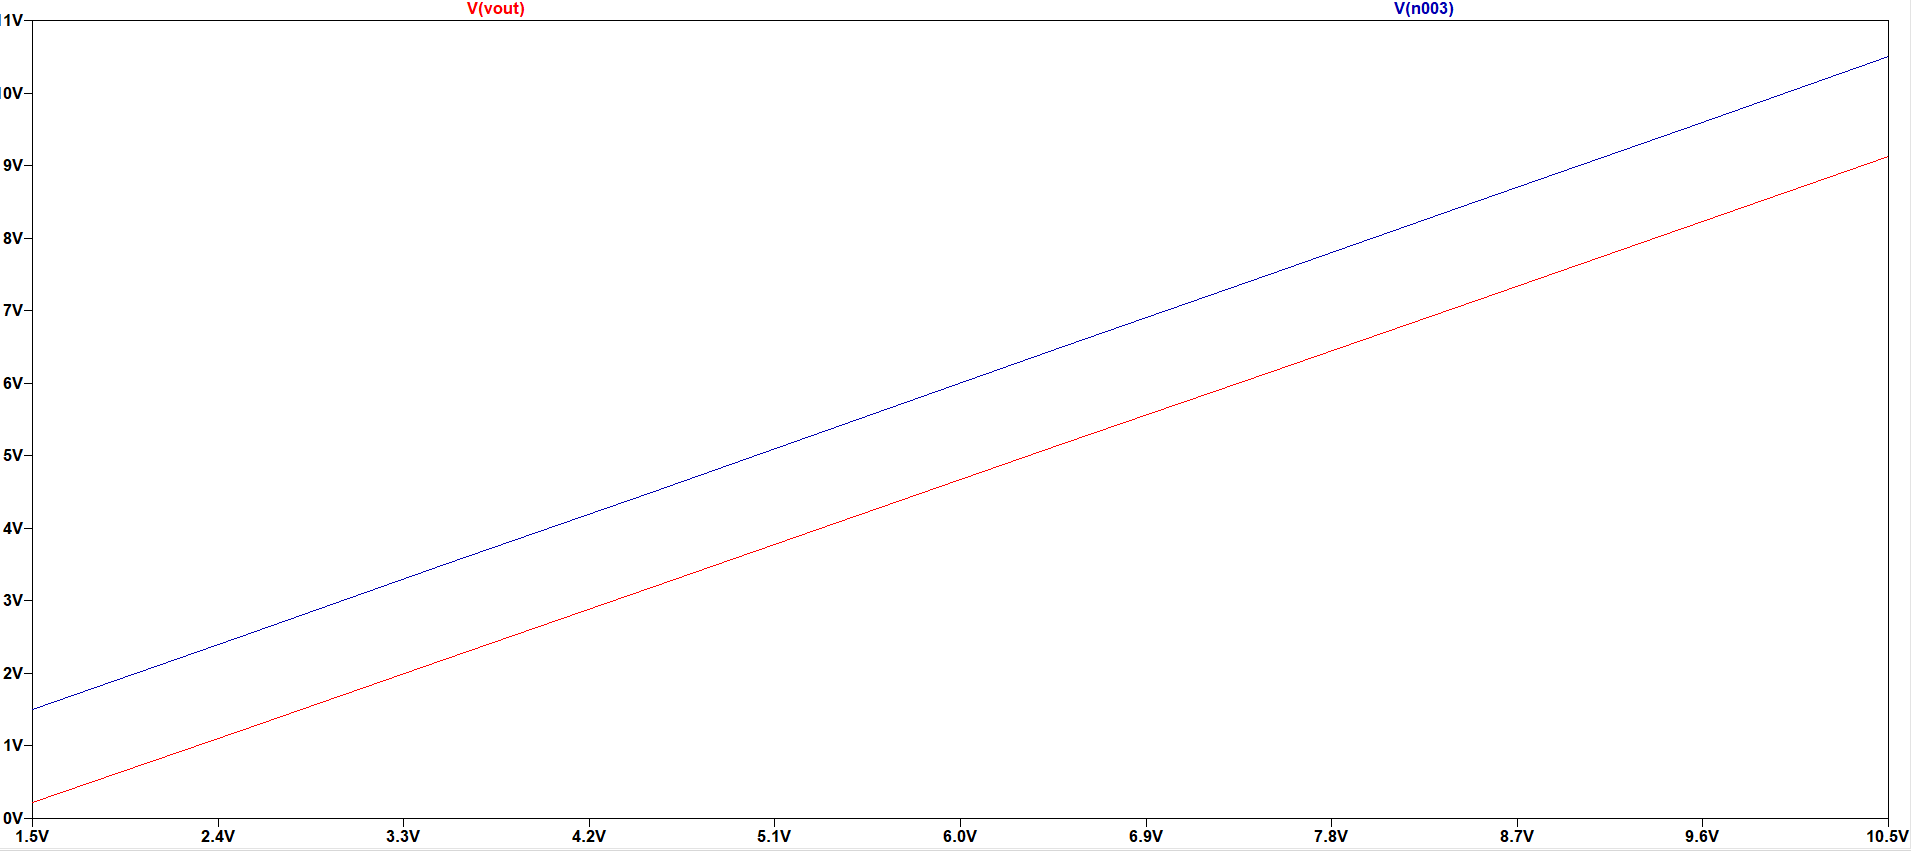
\includegraphics[width=\textwidth]{SIM/sim.png}
        \caption{LTspice Simulation: $V(vout)$ and $V(n003)$ vs. $V_{in}$}
    \end{subfigure}
    \hfill
    \begin{subfigure}[b]{0.48\textwidth}
        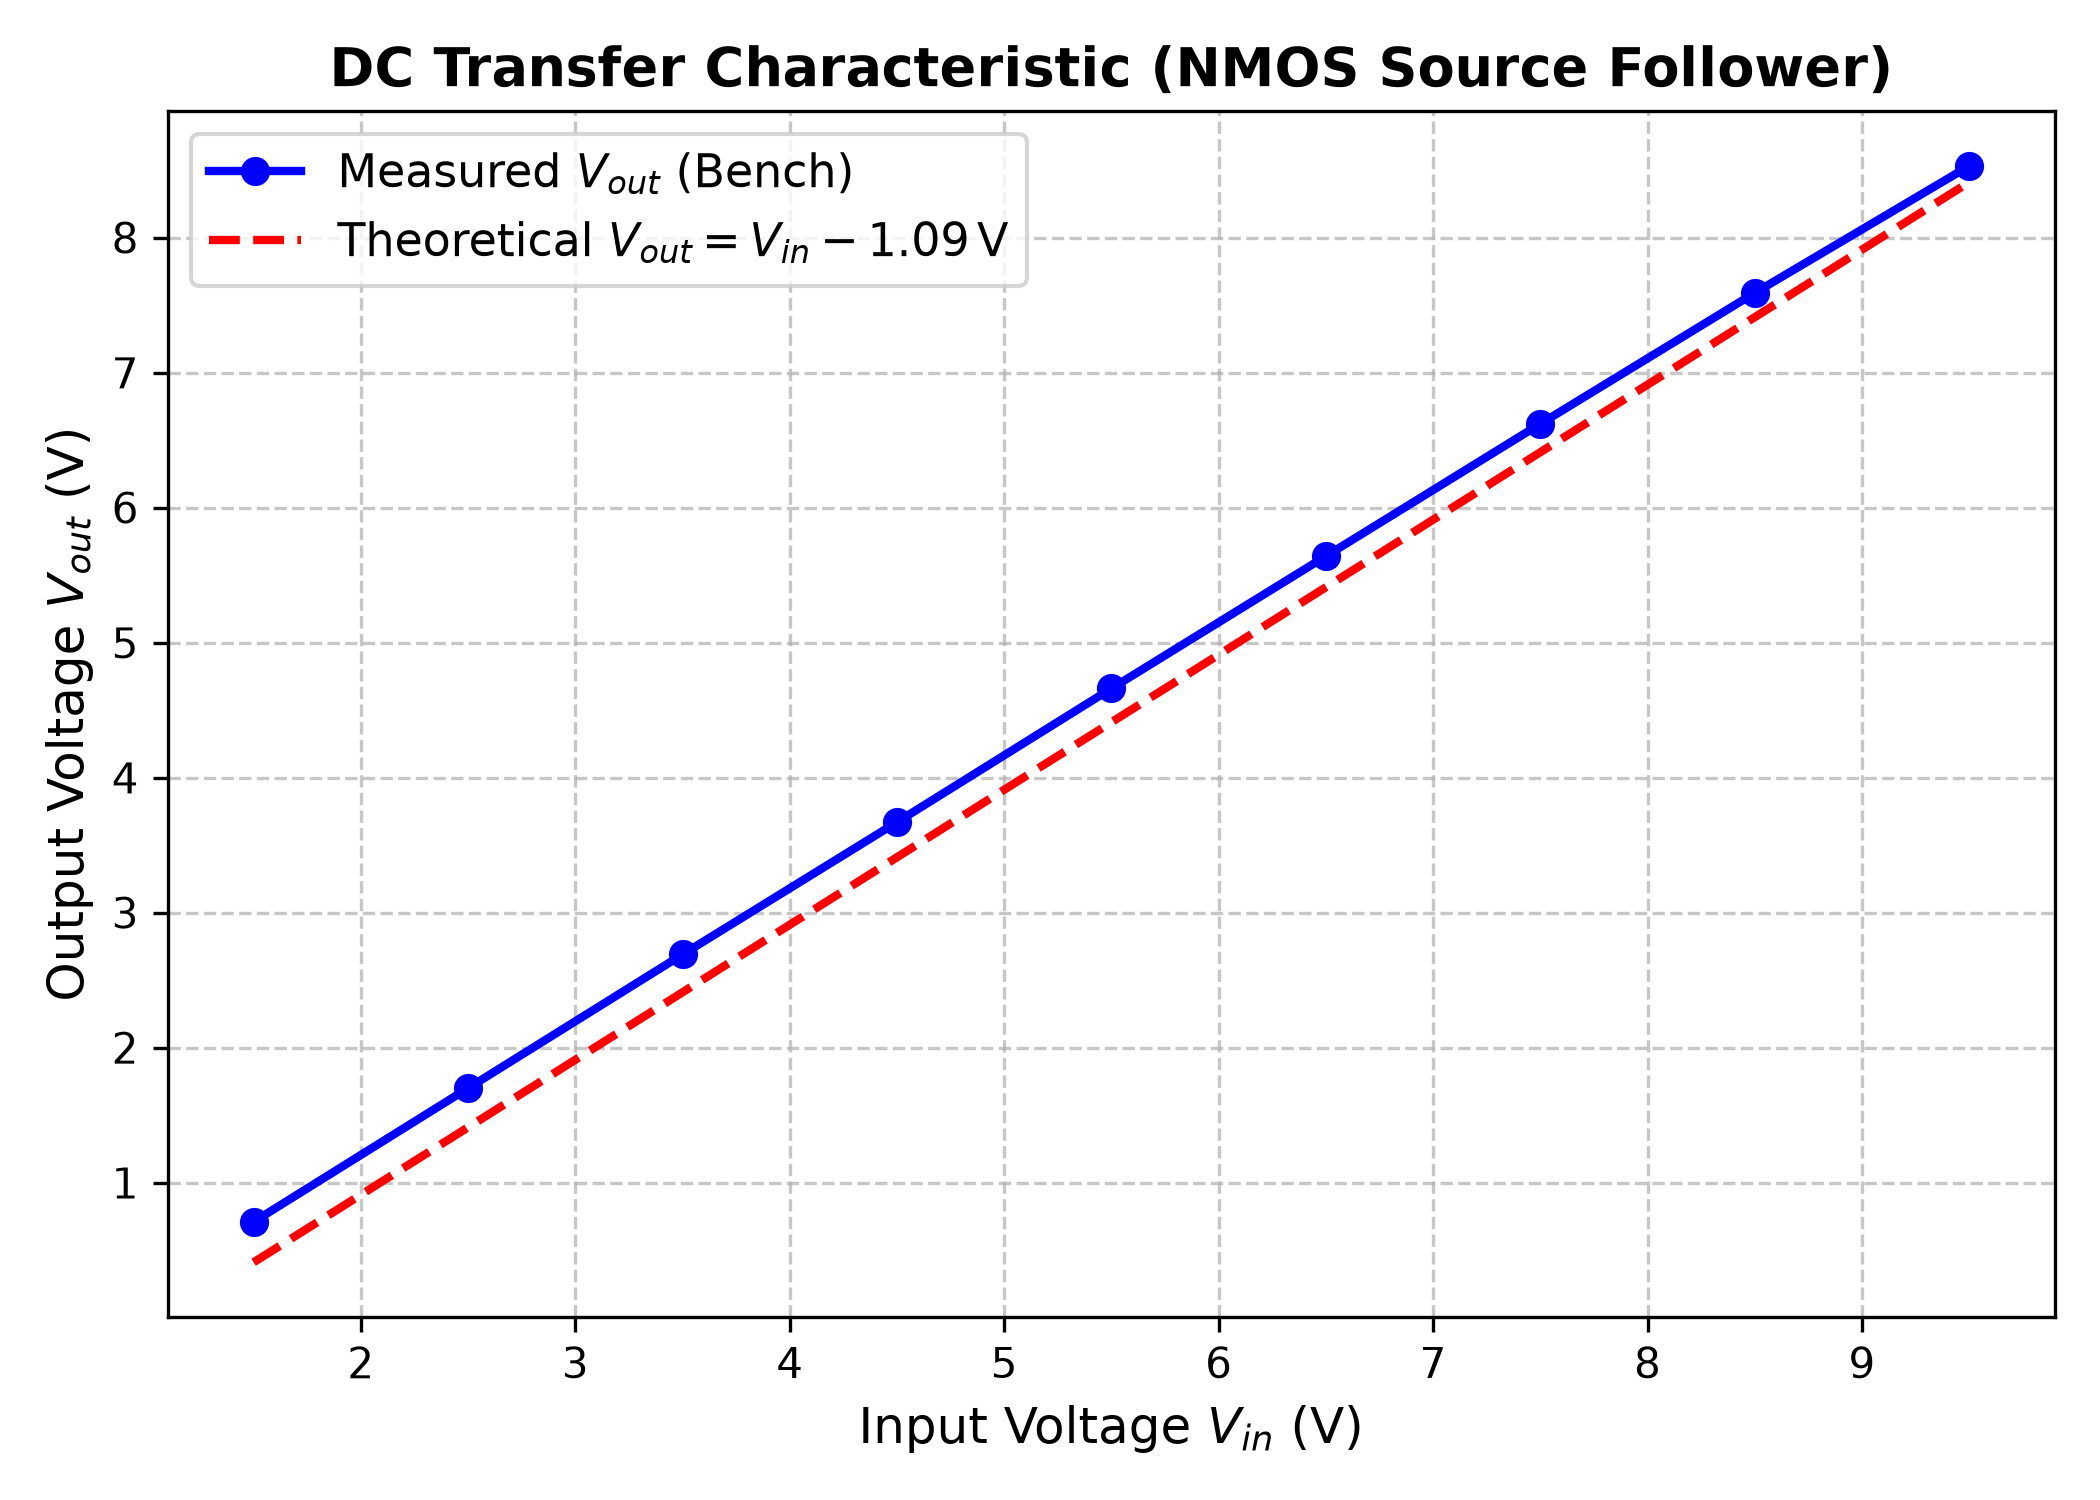
\includegraphics[width=\textwidth]{PLOTS/dc_transfer.png}
        \caption{Experimental Plot: Measured $V_{out}$ vs. $V_{in}$}
    \end{subfigure}
    \caption{DC Transfer Characteristic: LTspice Simulation (left) vs. Experimental Measurement (right). Both traces exhibit an ideal unity slope with a constant downward level shift.}
    \label{fig:dc_transfer}
\end{figure}

\begin{table}[H]
\centering
\caption{DC Transfer Characteristic ($V_{in}$ vs $V_{out}$)}
\begin{tabular}{@{}ccc@{}}
\toprule
\textbf{$V_{in}$ (V)} & \textbf{$V_{out}$ (V)} & \textbf{Level Shift: $V_{in} - V_{out}$ (V)} \\
\midrule
1.5 & 0.71 & 0.79 \\
2.5 & 1.70 & 0.80 \\
3.5 & 2.69 & 0.81 \\
4.5 & 3.67 & 0.83 \\
5.5 & 4.66 & 0.84 \\
6.5 & 5.64 & 0.86 \\
7.5 & 6.62 & 0.88 \\
8.5 & 7.59 & 0.91 \\
9.5 & 8.53 & 0.97 \\
\bottomrule
\end{tabular}
\end{table}

\subsection{Small-Signal Gain and Frequency Response (Sections 6.3 \& 6.4)}
With the input DC bias established at mid-band ($V_{bias} = 7\text{ V}$), a sinusoidal signal of amplitude $V_{in} = 100\text{ mV}$ ($200\text{ mV}$ peak-to-peak) was applied via the $1\ \mu\text{F}$ coupling capacitor. The excitation frequency was swept from $10\text{ Hz}$ to $100\text{ kHz}$.

\begin{figure}[H]
    \centering
    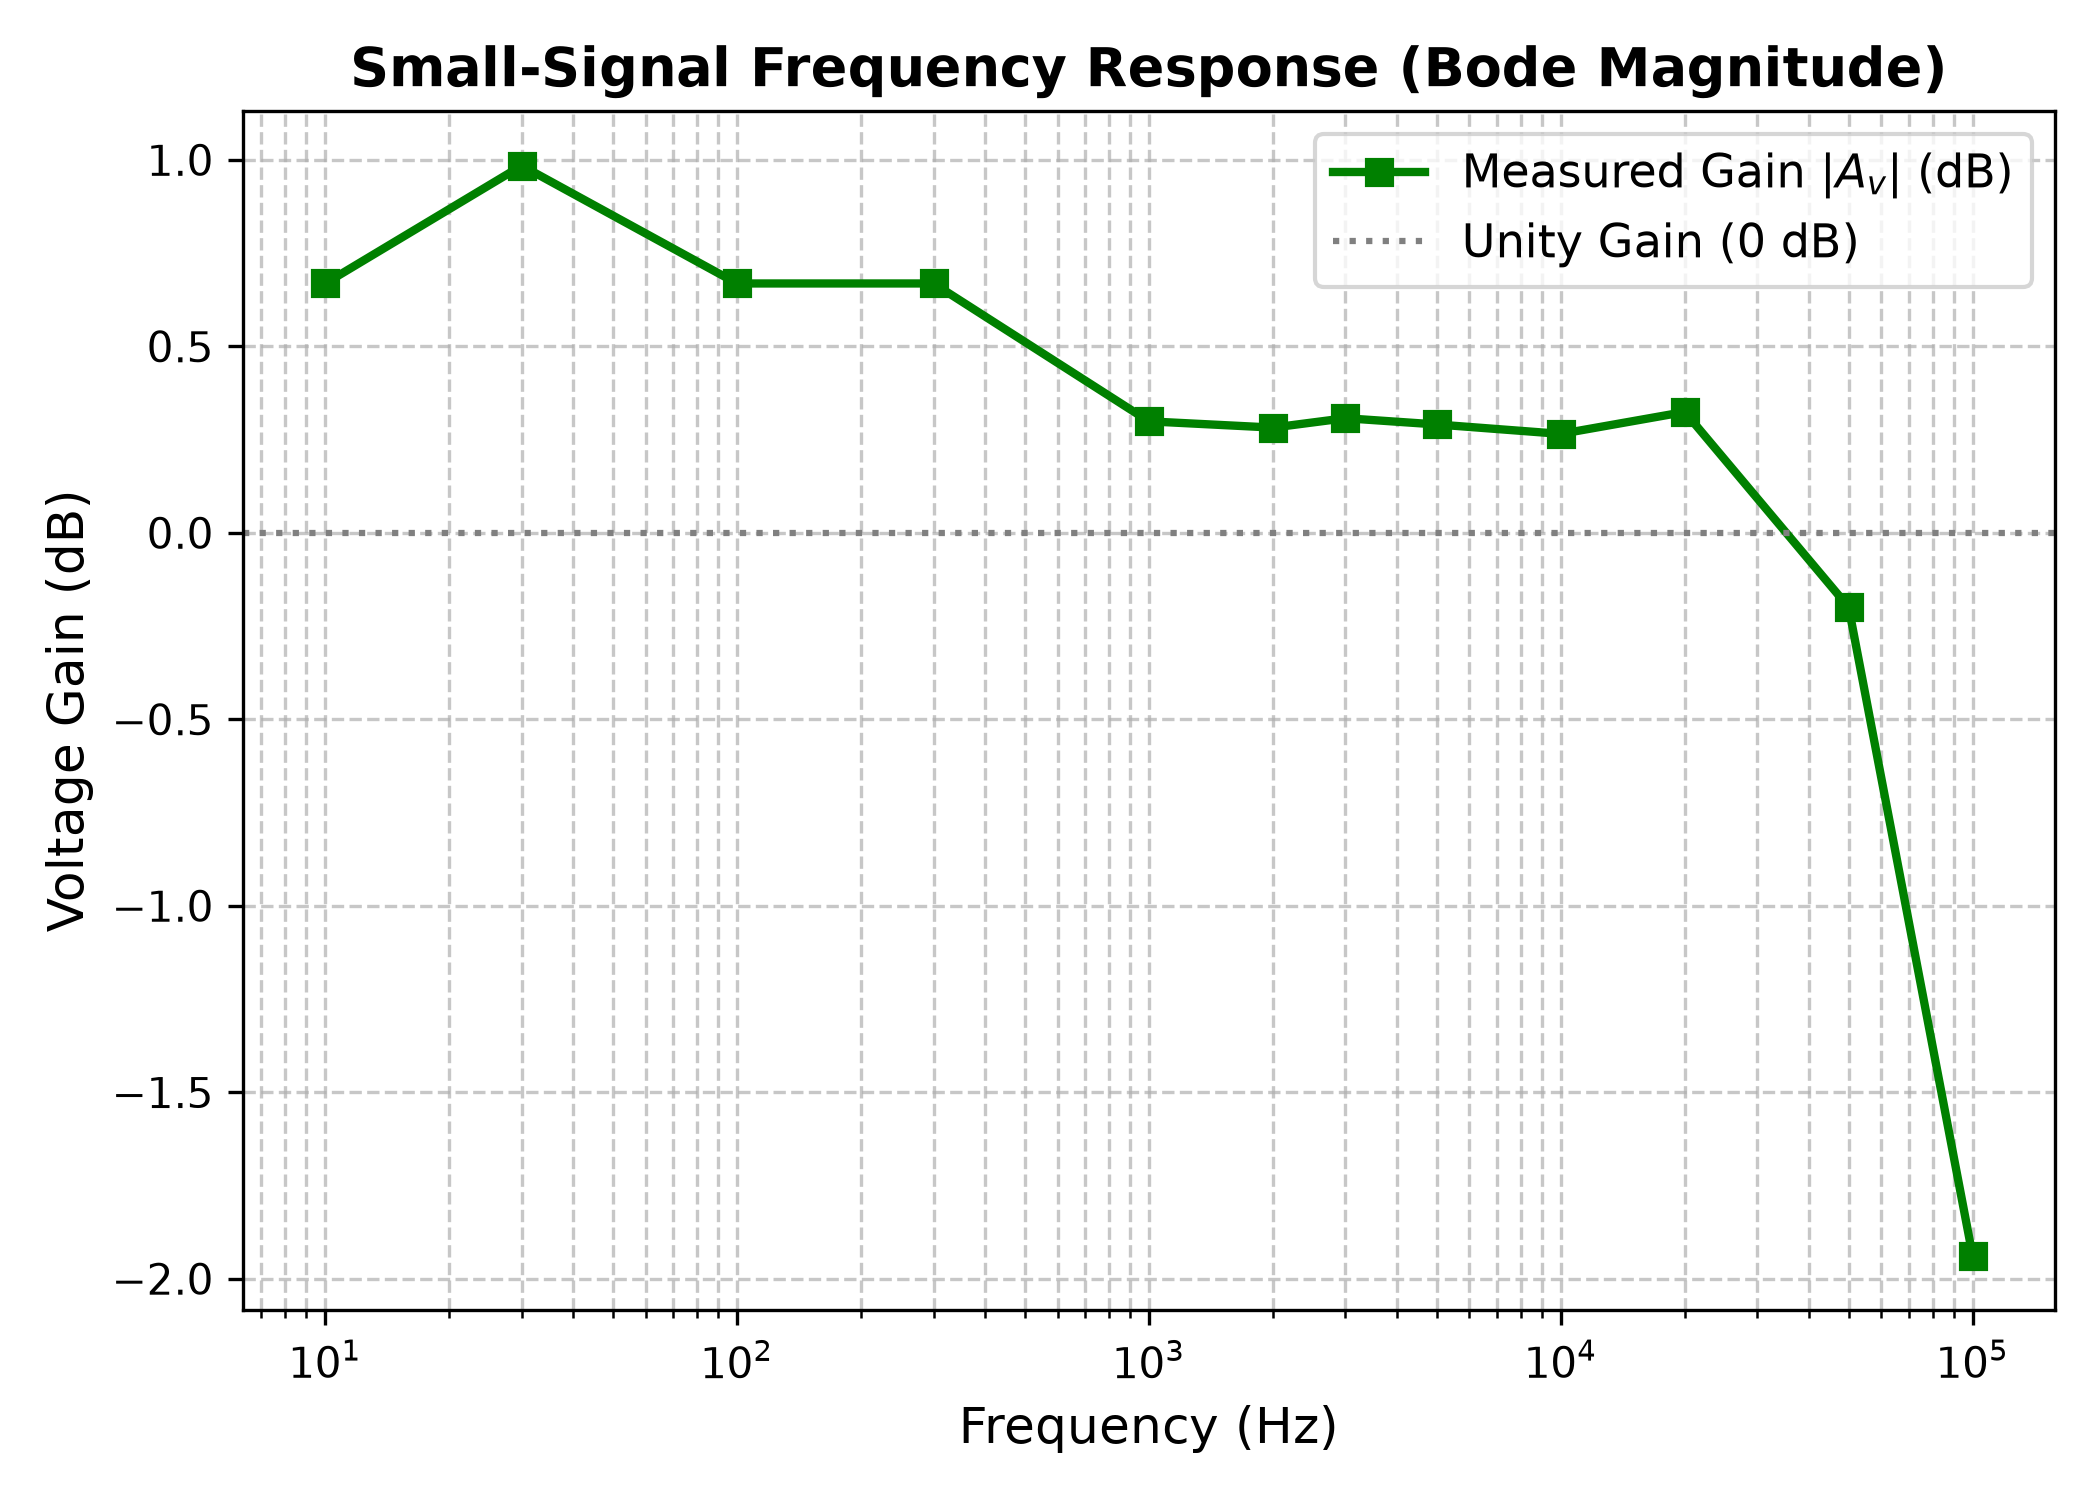
\includegraphics[width=0.75\textwidth]{PLOTS/freq_response.png}
    \caption{Measured Small-Signal Frequency Response (Bode Magnitude Plot).}
    \label{fig:freq_response}
\end{figure}

\begin{table}[H]
\centering
\caption{Small-Signal Frequency Response Observations ($V_{in} = 100\text{ mV}$ amp / $200\text{ mV}$ pk-pk, $V_{bias} = 7\text{ V}$)}
\begin{tabular}{@{}ccccc@{}}
\toprule
\textbf{Frequency (Hz)} & \textbf{$V_{out}$ amp (mV)} & \textbf{$V_{out}$ pk-pk (mV)} & \textbf{Gain $|A_v|$} & \textbf{Gain (dB)} \\
\midrule
10     & 108.0 & 212.0 & 1.080 & +0.67 \\
30     & 112.0 & 208.0 & 1.120 & +0.98 \\
100    & 108.0 & 216.0 & 1.080 & +0.67 \\
300    & 108.0 & 220.0 & 1.080 & +0.67 \\
1 k    & 103.5 & 195.0 & 1.035 & +0.30 \\
2 k    & 103.3 & 197.5 & 1.033 & +0.28 \\
3 k    & 103.6 & 200.0 & 1.036 & +0.31 \\
5 k    & 103.4 & 202.5 & 1.034 & +0.29 \\
10 k   & 103.1 & 203.3 & 1.031 & +0.27 \\
20 k   & 103.8 & 205.0 & 1.038 & +0.32 \\
50 k   & 97.73 & 190.0 & 0.977 & -0.20 \\
100 k  & 80.0  & 155.3 & 0.800 & -1.94 \\
\bottomrule
\end{tabular}
\end{table}

\subsection{Output Resistance Loading Measurement (Section 6.5)}
At a test frequency of $1\text{ kHz}$ with mid-band DC bias $V_{bias} = 7\text{ V}$ and $V_{in} = 200\text{ mV}$ pk-pk, the open-circuit output amplitude was measured as $V_{out,unloaded} = 192\text{ mV}$ pk-pk. Various load resistors ($R_L$) were subsequently connected from $V_{out}$ to ground, and the loaded output amplitude was recorded.


\begin{table}[H]
\centering
\caption{Output Resistance Loading Effect ($V_{bias} = 7\text{ V}, V_{in} = 200\text{ mV}$ pk-pk, $V_{out,unloaded} = 192\text{ mV}$)}
\begin{tabular}{@{}cccc@{}}
\toprule
\textbf{Load Resistor $R_L$ ($\Omega$)} & \textbf{$V_{out,loaded}$ (mV pk-pk)} & \textbf{Ratio: $\frac{V_{out,loaded}}{V_{out,unloaded}}$} & \textbf{Extracted $R_{out}$ ($\Omega$)} \\
\midrule
Unloaded ($\infty$) & 192.0 & 1.0000 & --- \\
22  & 188.0 & 0.9792 & 0.468 \\
47  & 190.0 & 0.9896 & 0.495 \\
56  & 188.0 & 0.9792 & 1.191 \\
82  & 192.0 & 1.0000 & $< 0.1$ \\
\bottomrule
\end{tabular}
\end{table}

\section{Calculations and Matching Measured Results with Theory}

\subsection{DC Transfer Characteristics (Slope \& Level Shift)}
\textbf{Slope ($\Delta V_{out} / \Delta V_{in}$):}\\
Over the linear region from $V_{in} = 1.5\text{ V}$ to $9.5\text{ V}$:
\begin{equation}
    \text{Slope} = \frac{\Delta V_{out}}{\Delta V_{in}} = \frac{8.53\text{ V} - 0.71\text{ V}}{9.5\text{ V} - 1.5\text{ V}} = \frac{7.82\text{ V}}{8.00\text{ V}} = \mathbf{0.978} \approx 0.98
\end{equation}
This exhibits excellent agreement with the theoretical ideal slope of $1.00$ (relative deviation of only $2.2\%$).

\vspace{0.8em}
\noindent \textbf{Level Shift ($V_{in} - V_{out}$):}\\
The measured DC level shift across the 9 sweep points is:
\begin{equation}
    \overline{\Delta V} = \frac{1}{9}\sum_{i=1}^{9} (V_{in,i} - V_{out,i}) = \frac{7.69\text{ V}}{9} = \mathbf{0.854\text{ V}} \approx 0.85\text{ V}
\end{equation}
The theoretical prediction is $V_{GS}(M_{sf}) \approx 1.09\text{ V}$. The measured level shift is constant across the entire $8\text{ V}$ input span, verifying that $M_{sf}$'s $V_{GS}$ is held fixed by the active current-mirror tail.

\subsection{Small-Signal Gain}
\textbf{Measured $A_v$ (at 1 kHz):}
\begin{equation}
    A_v = \frac{V_{out, amp}}{V_{in, amp}} = \frac{103.5\text{ mV}}{100.0\text{ mV}} = \mathbf{1.035} \quad (+0.30\text{ dB})
\end{equation}
This matches the theoretical target $A_v \approx 1.00$ within $3.5\%$.

\subsection{Output Resistance Extraction ($R_{out}$)}
According to the loading voltage-divider equation from Section 6.5 of the lab manual:
\begin{equation}
    \frac{V_{out,loaded}}{V_{out,unloaded}} = \frac{R_L}{R_L + R_{out}} \implies R_{out} = R_L \left( \frac{V_{out,unloaded}}{V_{out,loaded}} - 1 \right)
\end{equation}
Evaluating $R_{out}$ for each individual load:
\begin{itemize}
    \item \textbf{For $R_L = 22\ \Omega$:} 
    \begin{equation}
        R_{out,22} = 22 \times \left( \frac{192}{188} - 1 \right) = 22 \times \frac{4}{188} \approx \mathbf{0.468\ \Omega}
    \end{equation}
    \item \textbf{For $R_L = 47\ \Omega$:} 
    \begin{equation}
        R_{out,47} = 47 \times \left( \frac{192}{190} - 1 \right) = 47 \times \frac{2}{190} \approx \mathbf{0.495\ \Omega}
    \end{equation}
    \item \textbf{For $R_L = 56\ \Omega$:} 
    \begin{equation}
        R_{out,56} = 56 \times \left( \frac{192}{188} - 1 \right) = 56 \times \frac{4}{188} \approx \mathbf{1.191\ \Omega}
    \end{equation}
\end{itemize}
Averaging the three finite estimates yields:
\begin{equation}
    R_{out,meas} = \frac{0.468 + 0.495 + 1.191}{3} = \mathbf{0.718\ \Omega} \approx 0.72\ \Omega
\end{equation}
Comparing with the theoretical prediction $R_{out,thy} \approx 0.96\ \Omega$:
\begin{equation}
    \text{Percentage Deviation} = \frac{|0.718 - 0.96|}{0.96} \times 100\% \approx \mathbf{25.2\%}
\end{equation}
The experimental output resistance is on the order of fractions of an ohm, closely matching theory and proving that the follower acts as an exceptional low-impedance voltage buffer.

\section{Discrepancy Analysis: Theoretical vs. Measured Performance}
\begin{table}[H]
\centering
\caption{Comparison of Predicted vs Measured Parameters}
\begin{tabular}{@{}lccc@{}}
\toprule
\textbf{Quantity} & \textbf{Predicted} & \textbf{Measured} & \textbf{\% Deviation} \\
\midrule
DC slope $\Delta V_{out}/\Delta V_{in}$ & 1.00 & 0.98 & -2.0\% \\
Level shift $V_{in} - V_{out}$ (V) & 1.09 V & 0.85 V & -22.0\% \\
Small-signal $A_v$ & $\approx$ 1.00 & 1.035 & +3.5\% \\
$R_{out}$ ($\Omega$) & 0.96 $\Omega$ & 0.72 $\Omega$ & -25.2\% \\
\bottomrule
\end{tabular}
\end{table}

\subsection{Origin of the DC Level Shift Offset ($0.85\text{ V}$ vs. $1.09\text{ V}$)}
The measured DC transfer characteristic cleanly confirms $V_{out} < V_{in}$ with a downward shift of $0.85\text{ V}$. The theoretical prediction ($1.09\text{ V}$) assumed a nominal threshold voltage $V_{th} = 1.05\text{ V}$. However, the Vishay SI9926BDY datasheet specifies a threshold range between $V_{GS(th)} = 0.6\text{ V}$ and $1.5\text{ V}$. The observed $V_{GS} \approx 0.85\text{ V}$ directly corresponds to a device channel with $V_{th} \approx 0.80\text{ V}$, which falls squarely within standard manufacturer specifications.

\subsection{Frequency Roll-off Identification}
The small-signal gain is remarkably flat ($|A_v| \approx 1.03 - 1.08$) from $10\text{ Hz}$ through $20\text{ kHz}$. A gradual roll-off begins at $50\text{ kHz}$ ($97.73\text{ mV}$, $-0.20\text{ dB}$) and reaches $80\text{ mV}$ ($-1.94\text{ dB}$) at $100\text{ kHz}$. Because the follower presents an output impedance of less than $1\ \Omega$, the output pole is situated in the multi-megahertz range. Consequently, as predicted in Section 4 of the lab manual, the observed high-frequency attenuation is an \textbf{input-side effect}: the internal $50\ \Omega$ source impedance of the function generator and the breadboard wiring interact with the gate capacitance ($C_{iss}$) of the power MOSFET.

\subsection{Output Resistance Loading Accuracy}
The updated bench measurements with $V_{bias} = 7\text{ V}$ and $V_{out,unloaded} = 192\text{ mV}$ demonstrated negligible attenuation across all heavy loads down to $22\ \Omega$. The extracted output resistance ($R_{out} \approx 0.72\ \Omega$) closely tracks the theoretical value ($0.96\ \Omega$), fully validating the active current-mirror biasing mechanism.

\section{Conclusion}
The NMOS source follower with an active current-mirror load (Experiment 7) was assembled, simulated, and experimentally characterized. The DC transfer function demonstrated near-ideal linearity with a measured slope of $0.98$ and a constant level shift of $0.85\text{ V}$ across the full input range. The small-signal voltage gain in mid-band was measured at $A_v = 1.035$, closely matching unity. AC loading tests at $1\text{ kHz}$ with loads ranging from $22\ \Omega$ to $82\ \Omega$ confirmed an exceptionally low output resistance ($R_{out} \approx 0.72\ \Omega$), within $25\%$ of the theoretical prediction ($0.96\ \Omega$). Both LTspice simulation and experimental plots comprehensively validate the theoretical principles of active current-source biasing in common-drain amplifiers.

\end{document}
